\section{Sensitivity Analysis}


\begin{figure*}[]  % Use [p] for a dedicated page
\centering
\caption{Sensitivity analysis of meta-heuristic performance across optimization strategies, hardware scale factors and area constraint}
\label{fig:sensitivity_all}

% Row 1: ARATO
\subfloat[ARATO, $k=0.1$]{%
    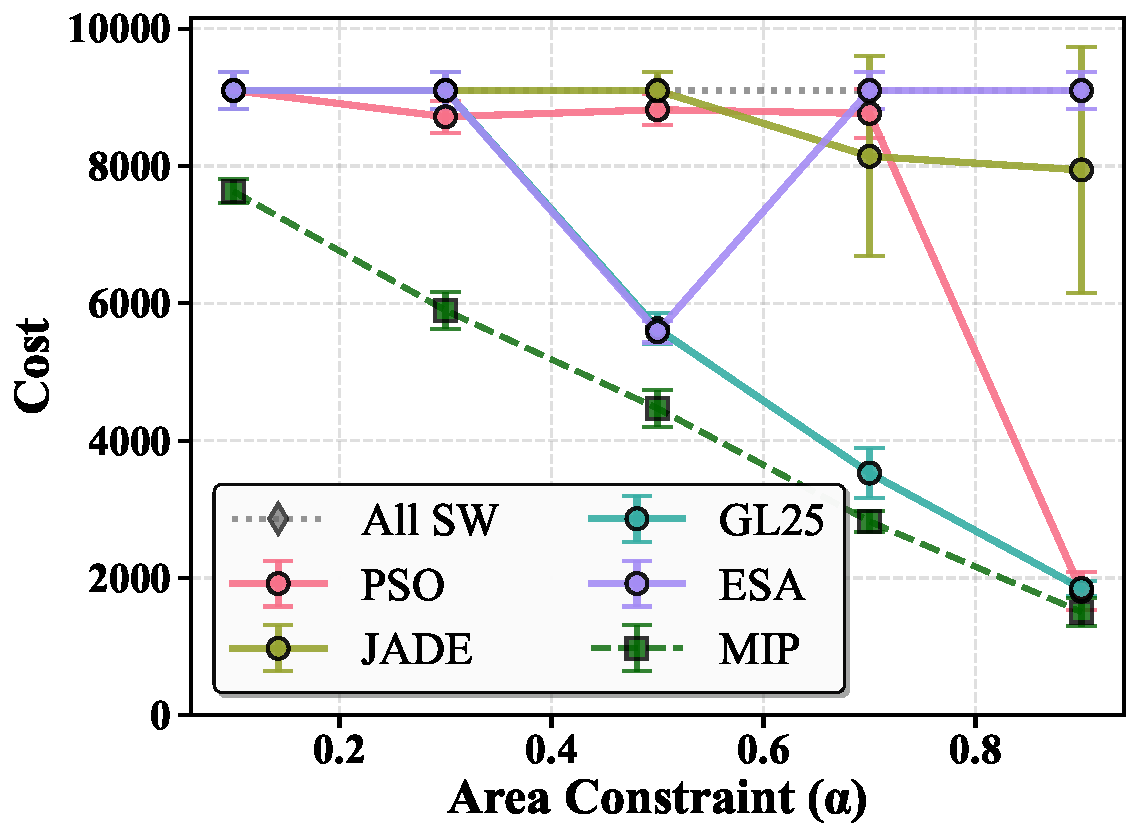
\includegraphics[width=0.32\textwidth]{Figures/meta-heuristic-Figures/sensitivity_methods_vs_area_hw_0.1_strategy_ARATO.pdf}
}\hfill
\subfloat[ARATO, $k=0.5$]{%
    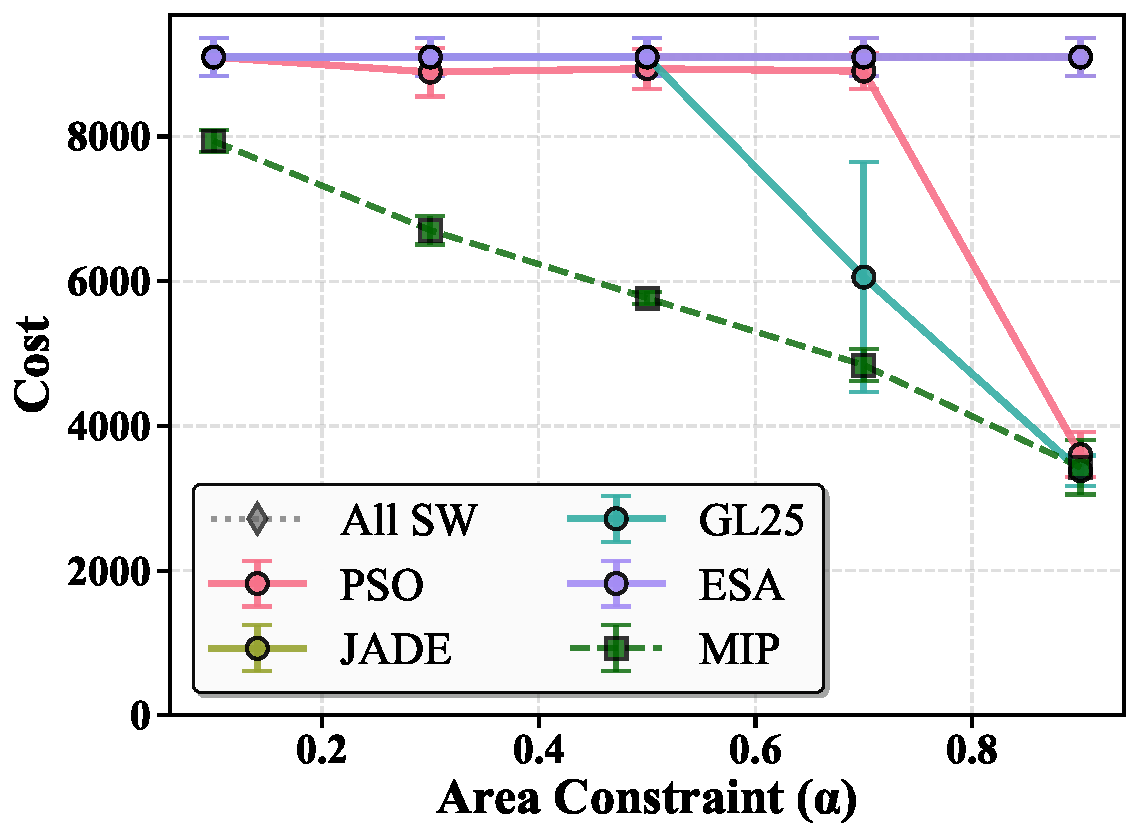
\includegraphics[width=0.32\textwidth]{Figures/meta-heuristic-Figures/sensitivity_methods_vs_area_hw_0.5_strategy_ARATO.pdf}
}\hfill
\subfloat[ARATO, $k=0.9$]{%
    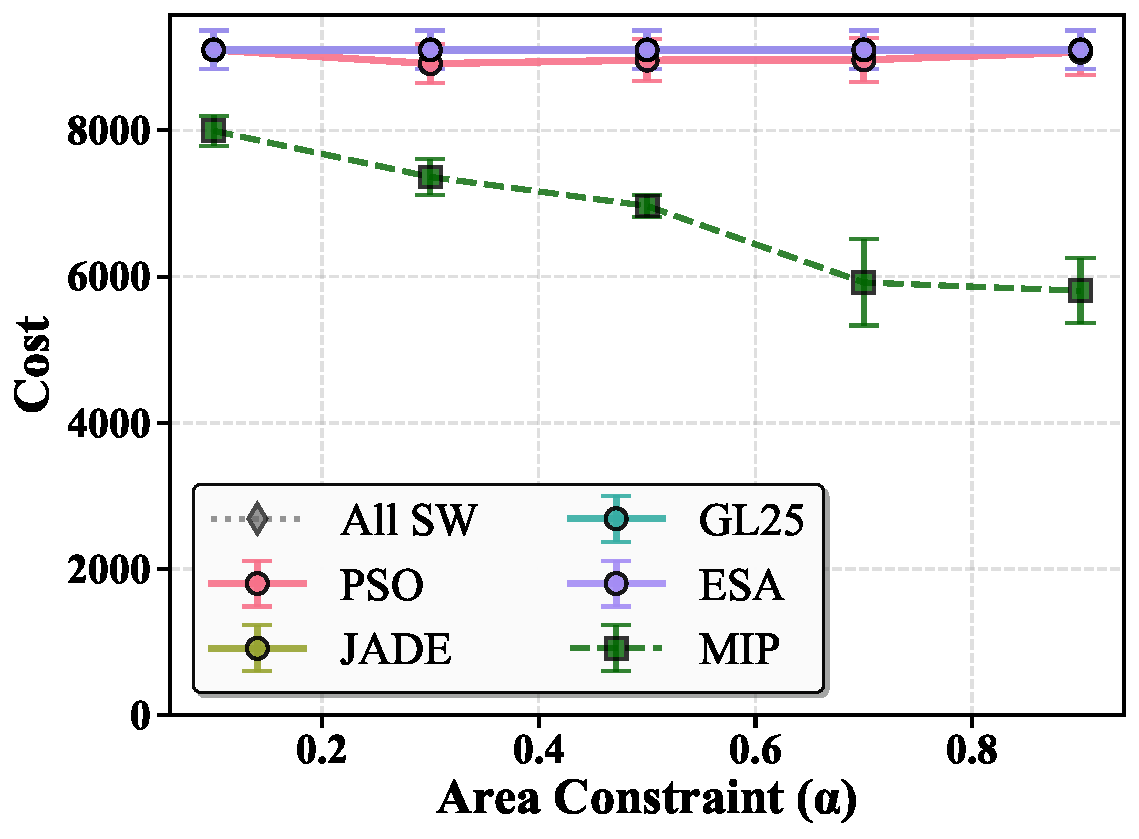
\includegraphics[width=0.32\textwidth]{Figures/meta-heuristic-Figures/sensitivity_methods_vs_area_hw_0.9_strategy_ARATO.pdf}
}\\

% Row 2: CA
\subfloat[CA, $k=0.1$]{%
    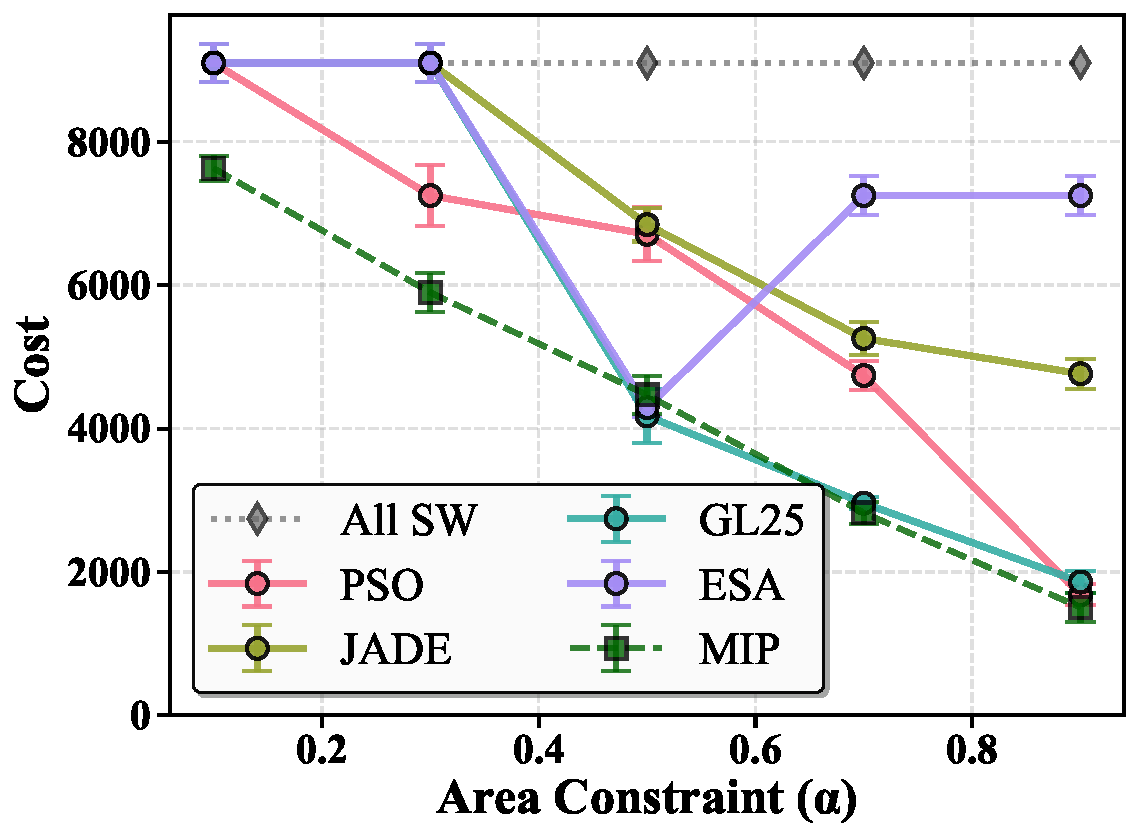
\includegraphics[width=0.32\textwidth]{Figures/meta-heuristic-Figures/sensitivity_methods_vs_area_hw_0.1_strategy_CA.pdf}
}\hfill
\subfloat[CA, $k=0.5$]{%
    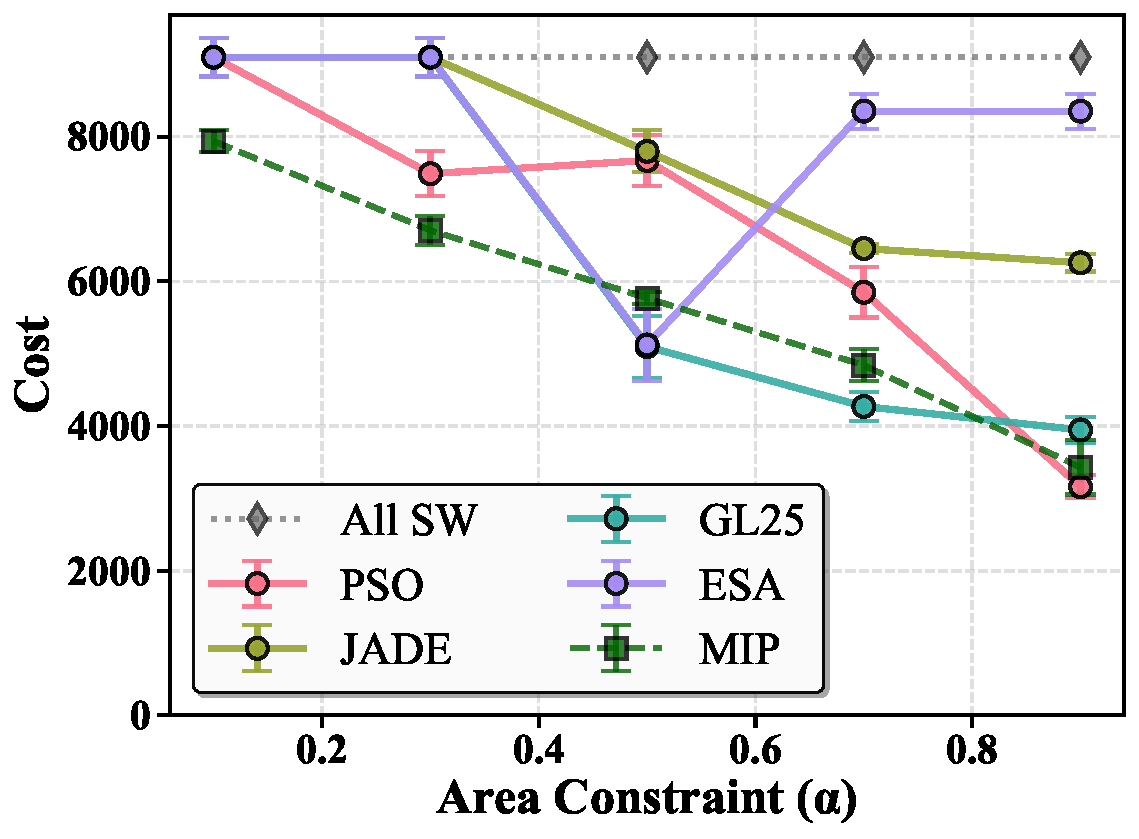
\includegraphics[width=0.32\textwidth]{Figures/meta-heuristic-Figures/sensitivity_methods_vs_area_hw_0.5_strategy_CA.pdf}
}\hfill
\subfloat[CA, $k=0.9$]{%
    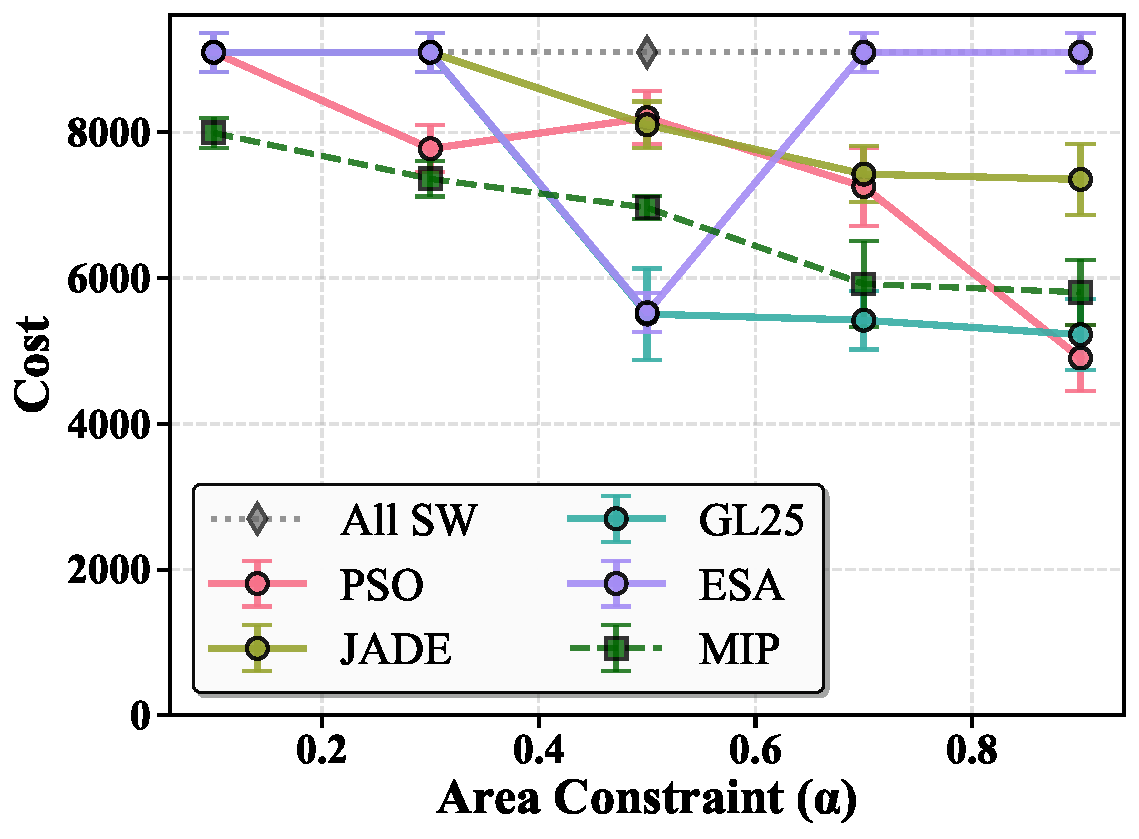
\includegraphics[width=0.32\textwidth]{Figures/meta-heuristic-Figures/sensitivity_methods_vs_area_hw_0.9_strategy_CA.pdf}
}\\

% Row 3: CPL
% \subfloat[CPL, $k=0.1$]{%
%     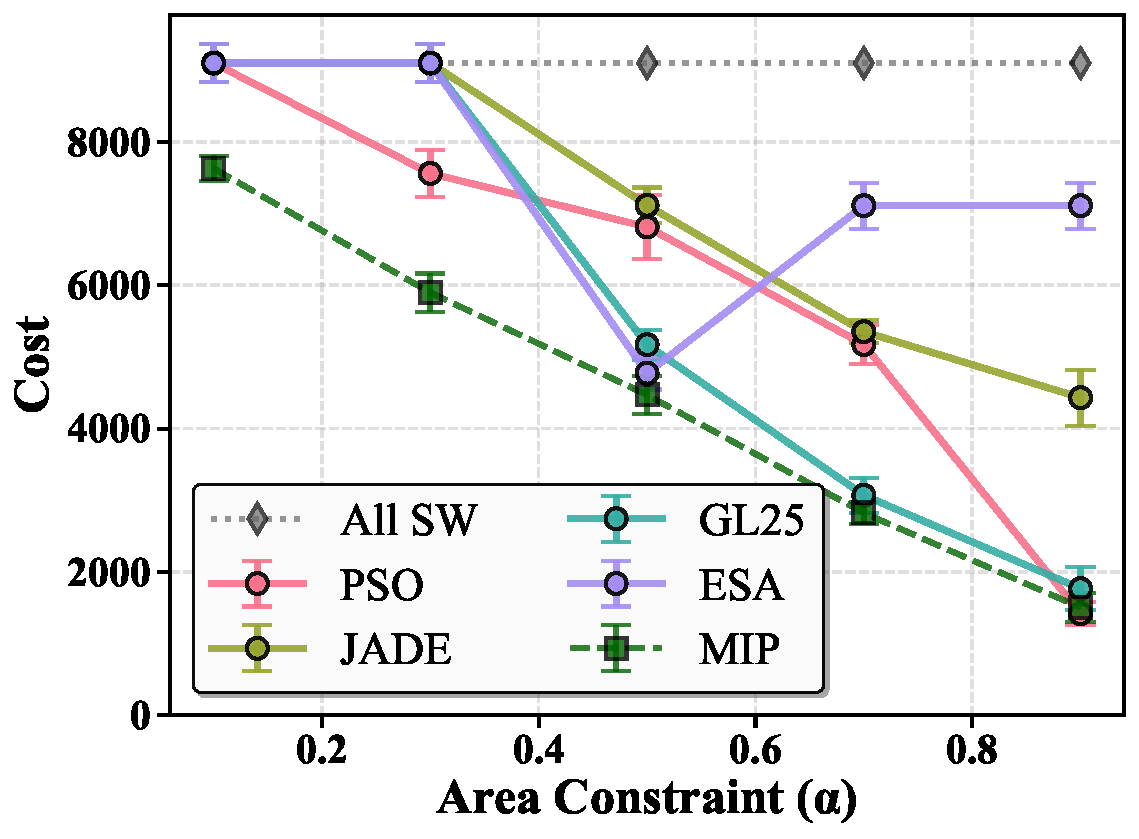
\includegraphics[width=0.32\textwidth]{Figures/meta-heuristic-Figures/sensitivity_methods_vs_area_hw_0.1_strategy_CPL.pdf}
% }\hfill
% \subfloat[CPL, $k=0.5$]{%
%     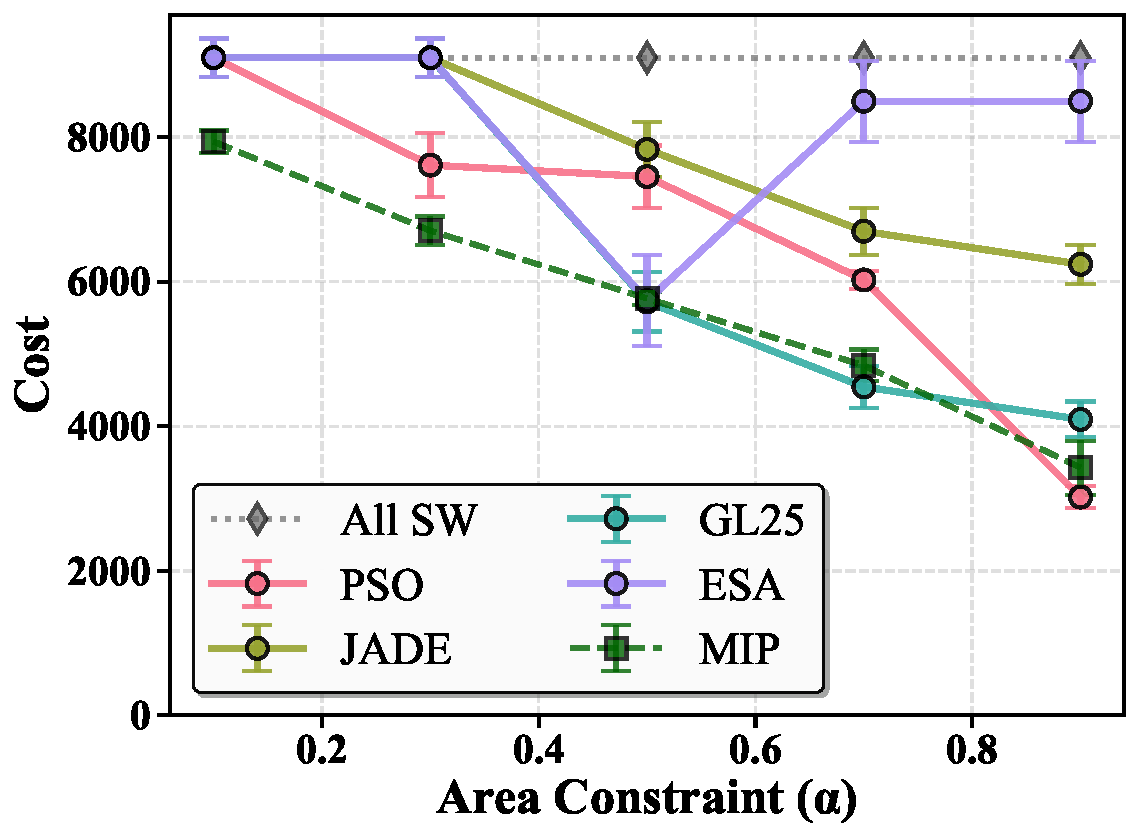
\includegraphics[width=0.32\textwidth]{Figures/meta-heuristic-Figures/sensitivity_methods_vs_area_hw_0.5_strategy_CPL.pdf}
% }\hfill
% \subfloat[CPL, $k=0.9$]{%
%     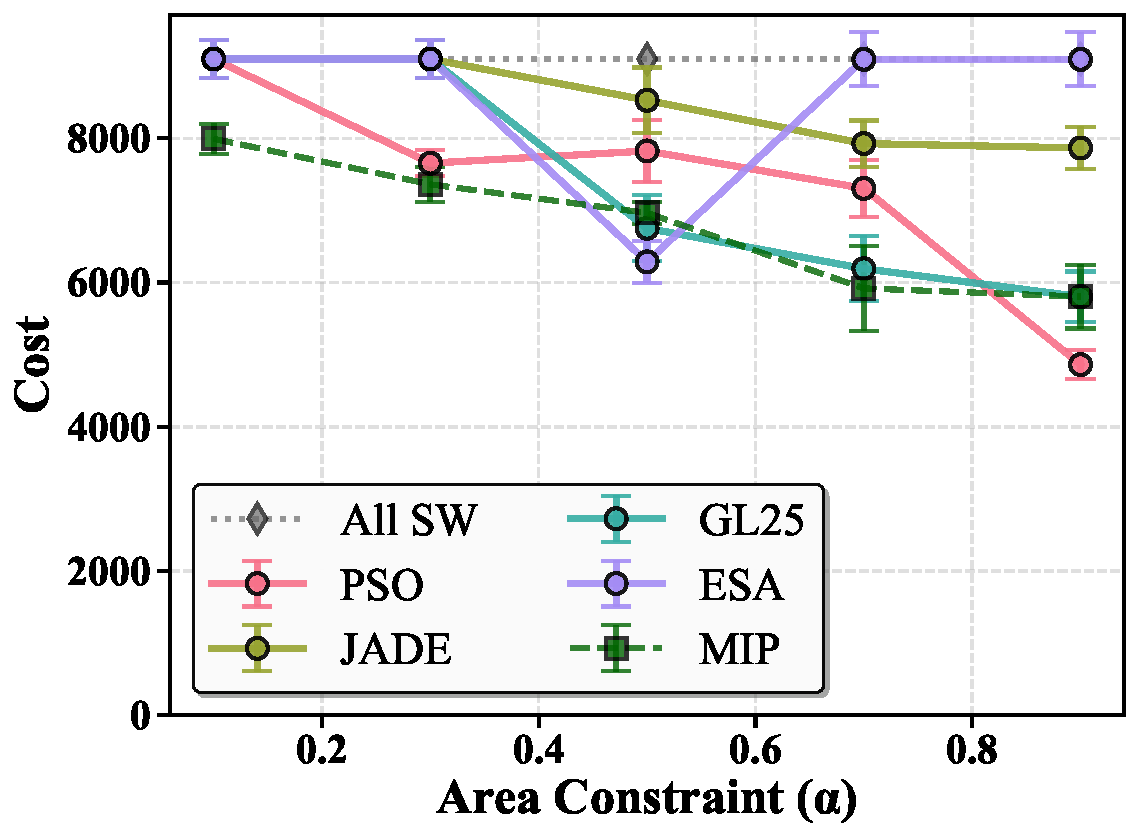
\includegraphics[width=0.32\textwidth]{Figures/meta-heuristic-Figures/sensitivity_methods_vs_area_hw_0.9_strategy_CPL.pdf}
% }\\

% % Row 4: ED
% \subfloat[ED, $k=0.1$]{%
%     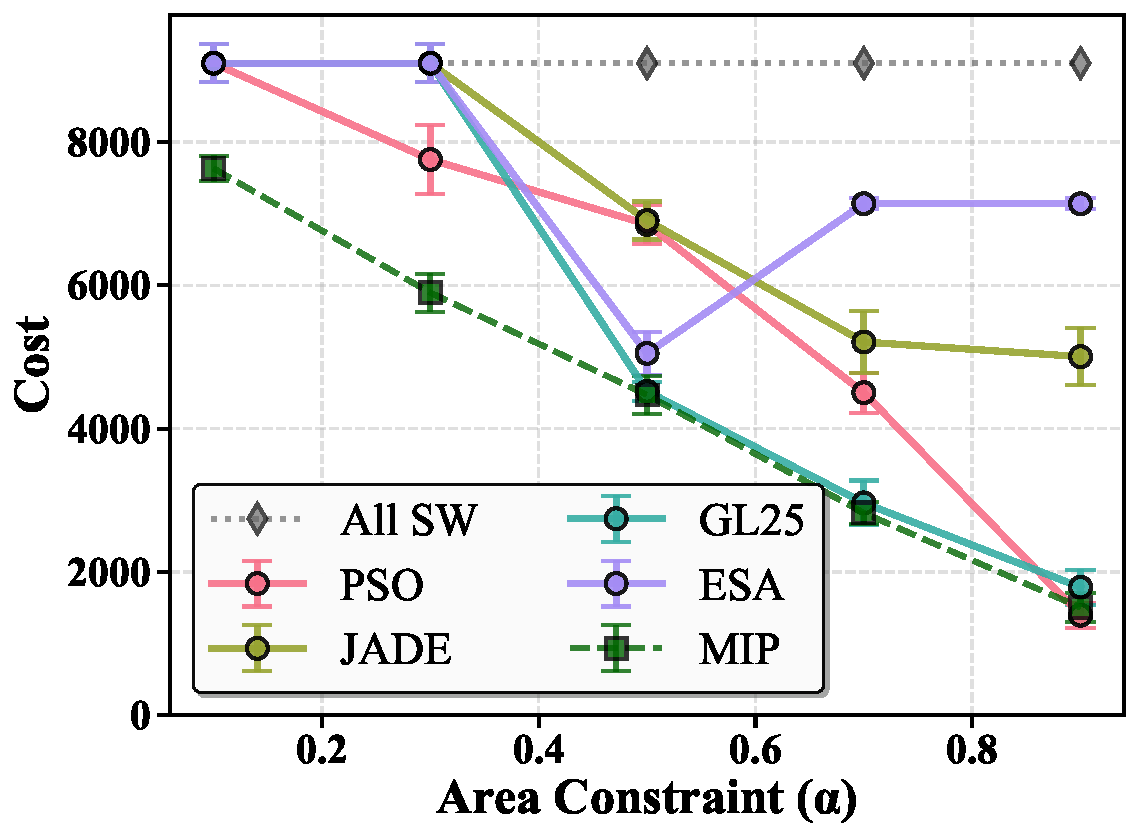
\includegraphics[width=0.32\textwidth]{Figures/meta-heuristic-Figures/sensitivity_methods_vs_area_hw_0.1_strategy_ED.pdf}
% }\hfill
% \subfloat[ED, $k=0.5$]{%
%     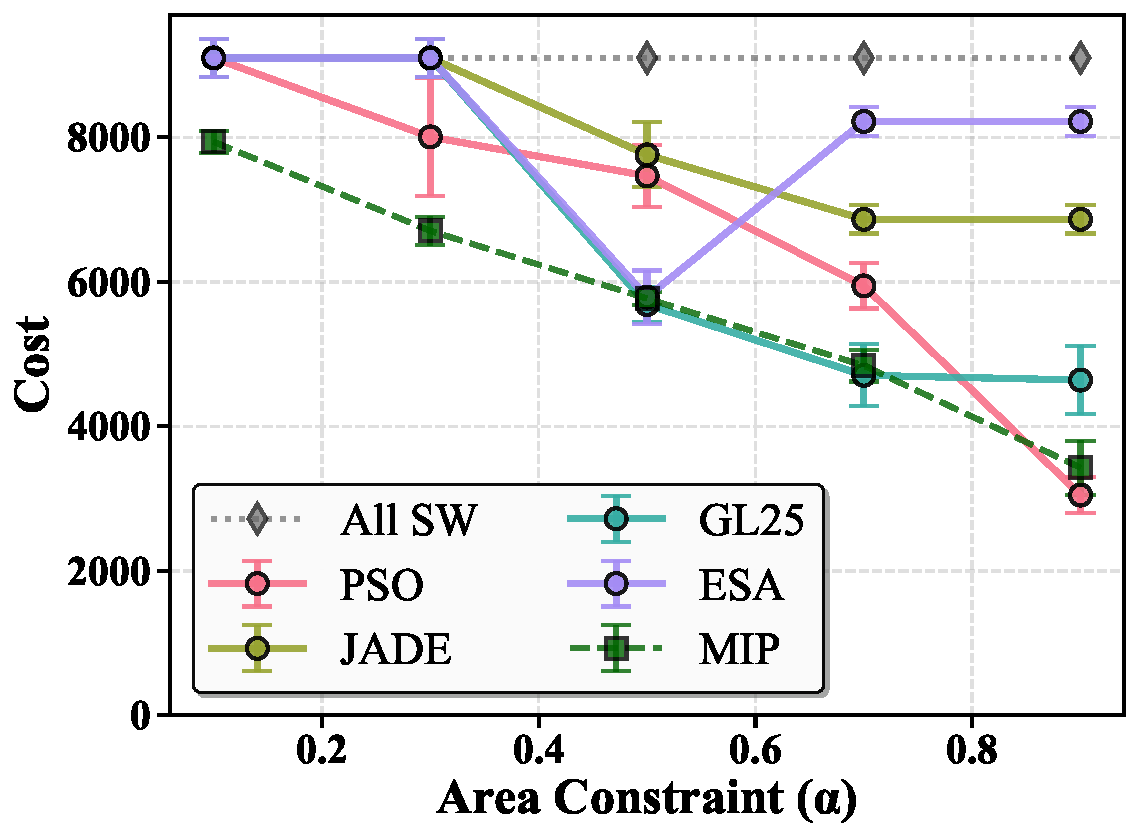
\includegraphics[width=0.32\textwidth]{Figures/meta-heuristic-Figures/sensitivity_methods_vs_area_hw_0.5_strategy_ED.pdf}
% }\hfill
% \subfloat[ED, $k=0.9$]{%
%     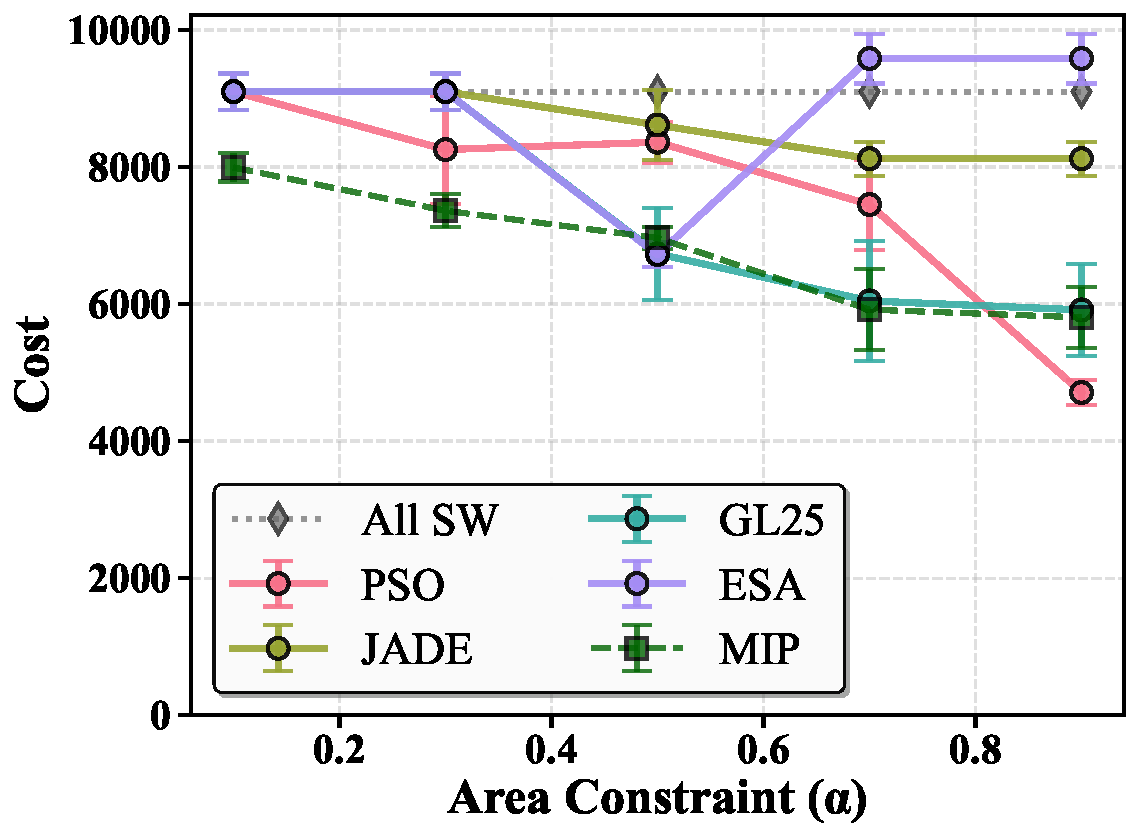
\includegraphics[width=0.32\textwidth]{Figures/meta-heuristic-Figures/sensitivity_methods_vs_area_hw_0.9_strategy_ED.pdf}
% }\\

% % Row 5: SPT
% \subfloat[SPT, $k=0.1$]{%
%     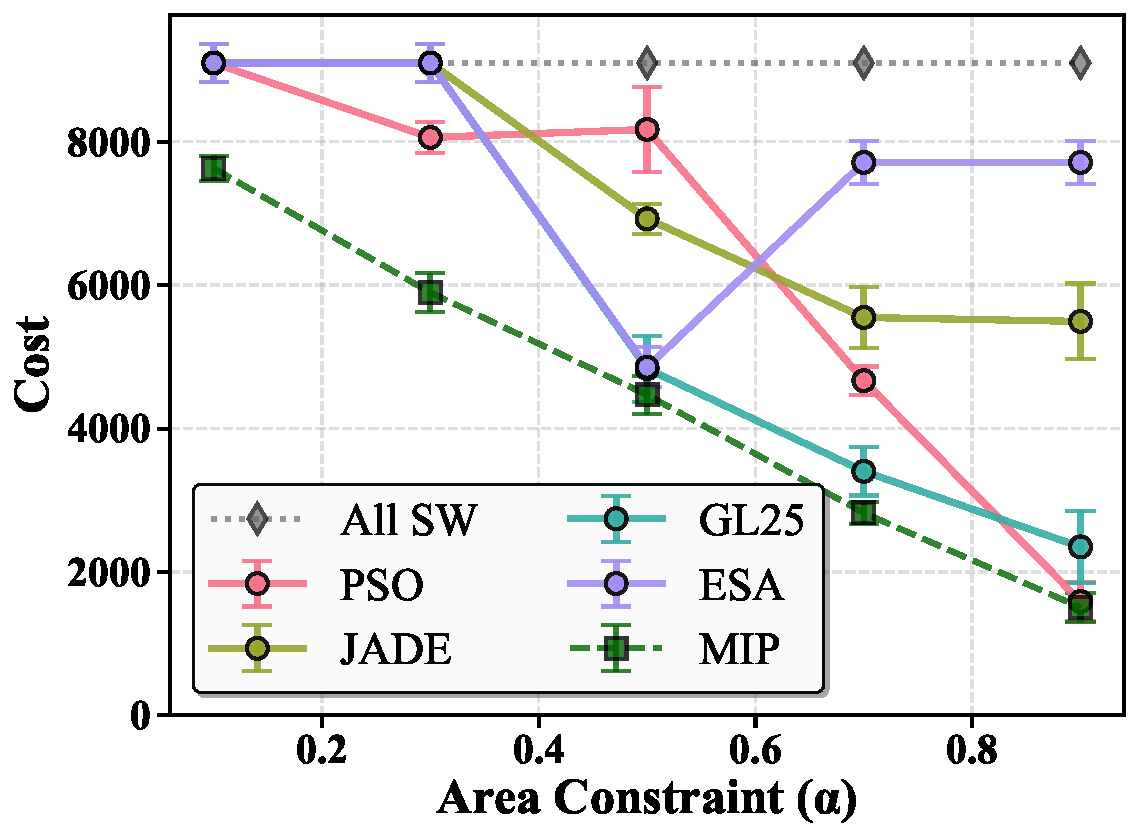
\includegraphics[width=0.32\textwidth]{Figures/meta-heuristic-Figures/sensitivity_methods_vs_area_hw_0.1_strategy_SPT.pdf}
% }\hfill
% \subfloat[SPT, $k=0.5$]{%
%     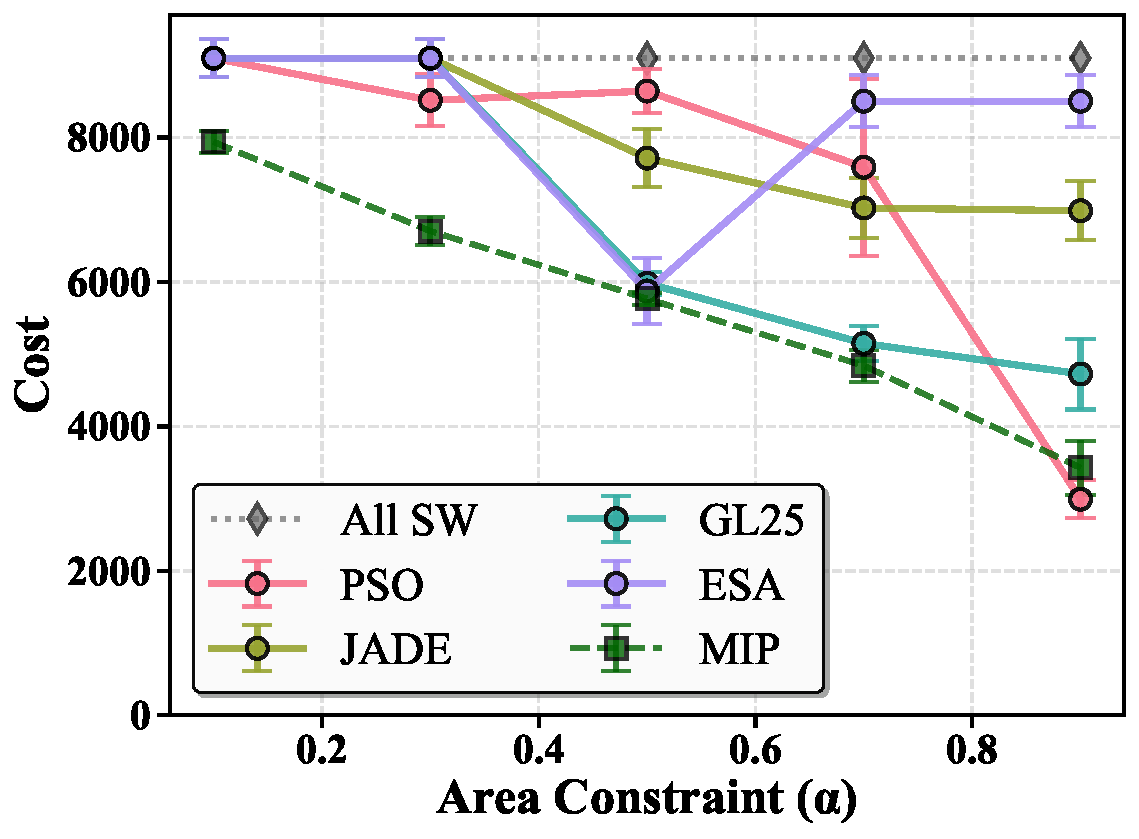
\includegraphics[width=0.32\textwidth]{Figures/meta-heuristic-Figures/sensitivity_methods_vs_area_hw_0.5_strategy_SPT.pdf}
% }\hfill
% \subfloat[SPT, $k=0.9$]{%
%     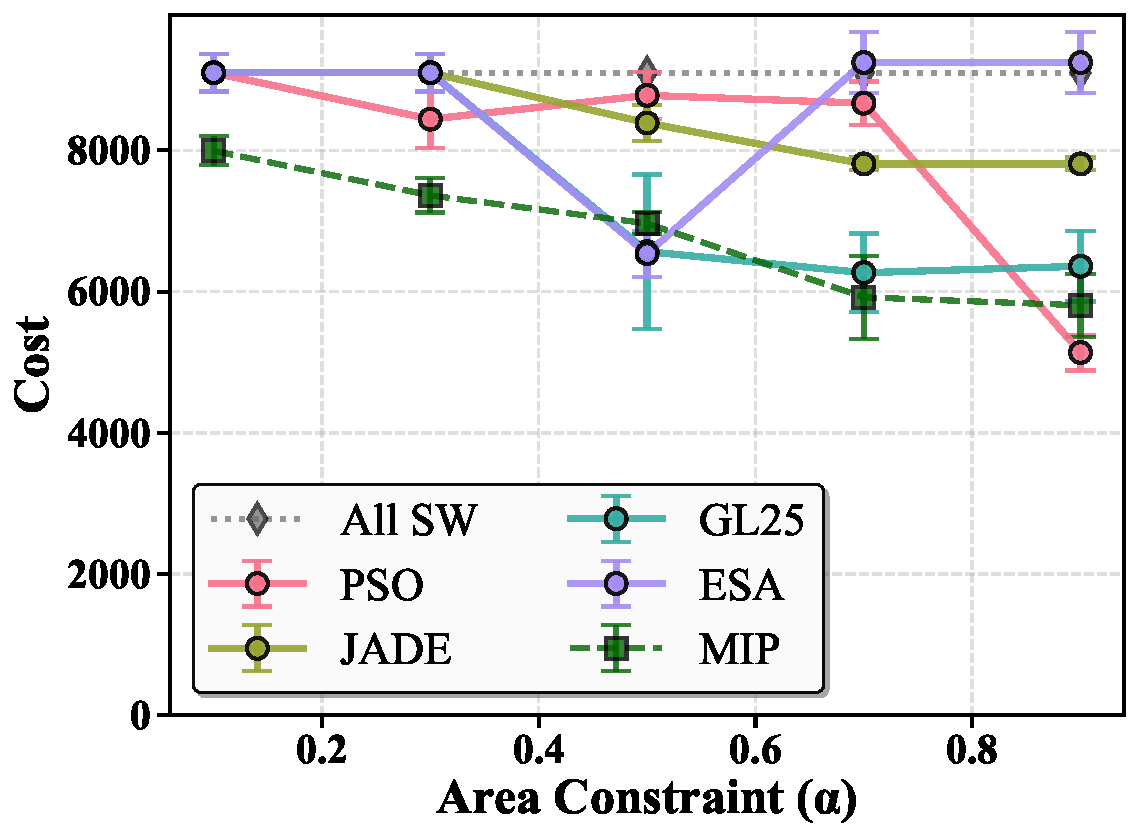
\includegraphics[width=0.32\textwidth]{Figures/meta-heuristic-Figures/sensitivity_methods_vs_area_hw_0.9_strategy_SPT.pdf}
% }\\

% Row 6: OPTM
% \subfloat[OPTM, $k=0.1$]{%
%     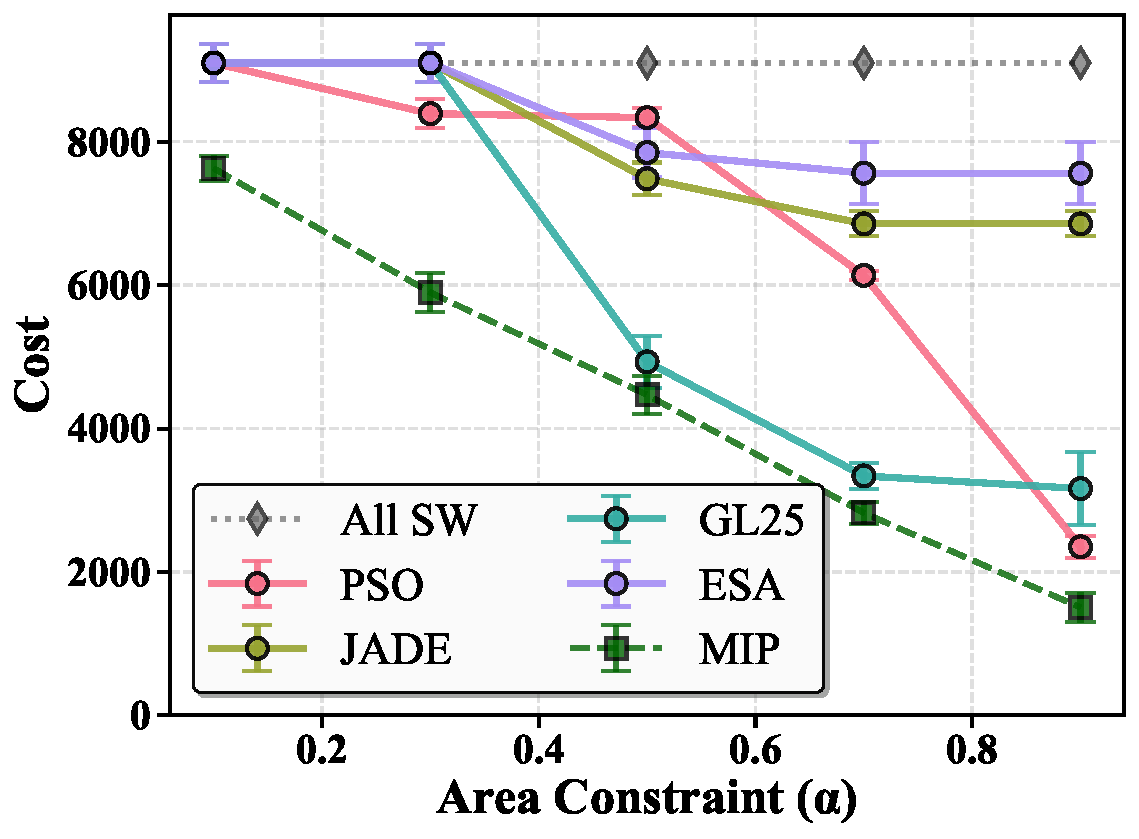
\includegraphics[width=0.32\textwidth]{Figures/meta-heuristic-Figures/sensitivity_methods_vs_area_hw_0.1_strategy_OPTM.pdf}
% }\hfill
% \subfloat[OPTM, $k=0.5$]{%
%     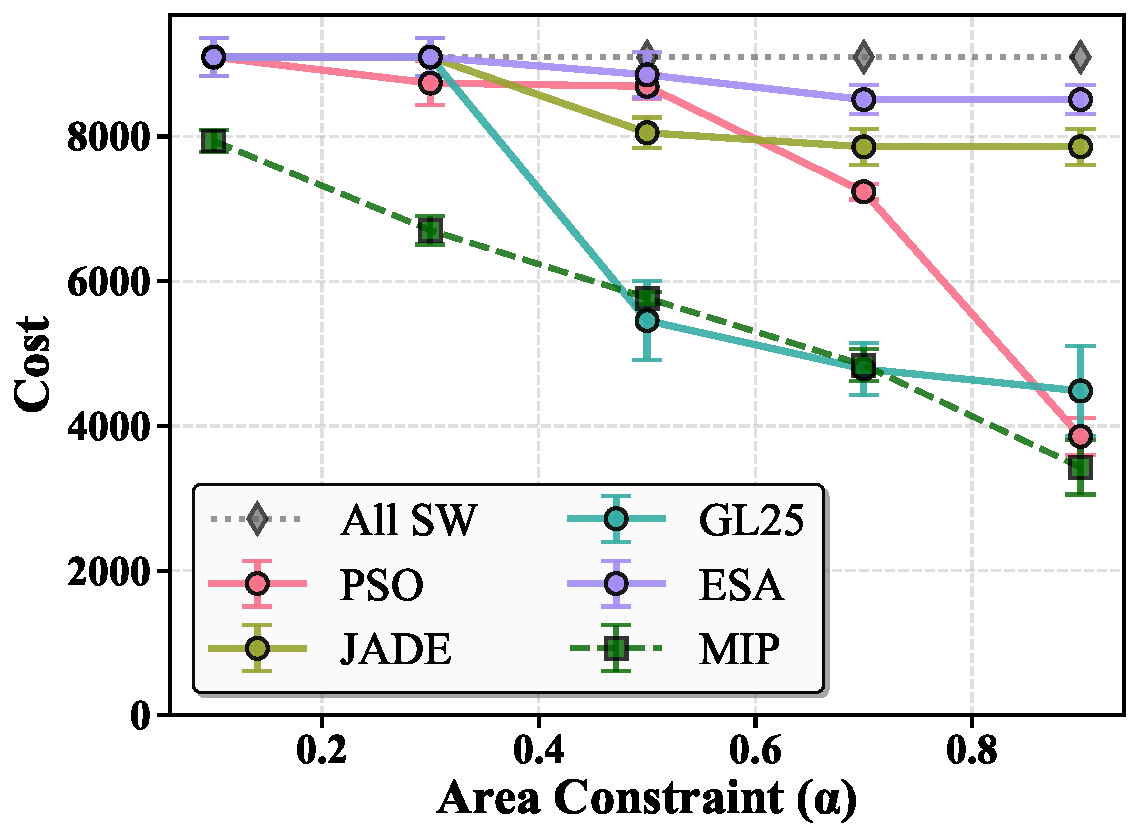
\includegraphics[width=0.32\textwidth]{Figures/meta-heuristic-Figures/sensitivity_methods_vs_area_hw_0.5_strategy_OPTM.pdf}
% }\hfill
% \subfloat[OPTM, $k=0.9$]{%
%     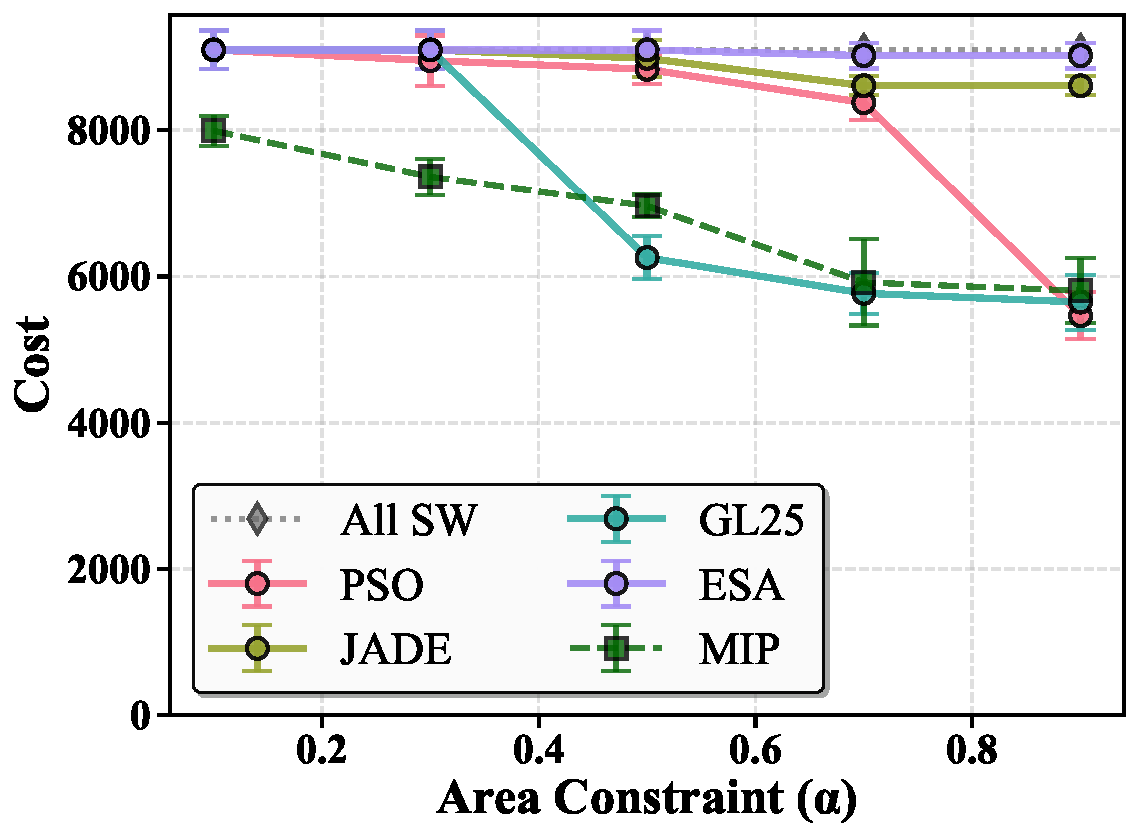
\includegraphics[width=0.32\textwidth]{Figures/meta-heuristic-Figures/sensitivity_methods_vs_area_hw_0.9_strategy_OPTM.pdf}
% }

\end{figure*}



This section presents a detailed sensitivity analysis of four meta-heuristic algorithms (PSO, JADE, GL25, ESA) against two baselines (MIP (expected best), naive all-software (expected worst)) across two optimization strategies and various hardware scale factors ($k \in \{0.1, 0.5, 0.9\}$) and area constraints ($\alpha \in \{0.1, 0.3, 0.5, 0.7, 0.9\}$).

\subsection{Optimization Strategy: ARATO}

At $k=0.1$ where hardware assignment provides a 10$\times$ speedup on average than the corresponding software assignment, the meta-heuristics exhibit significant differences in their performances when they use ARATO optimization strategy. GL25 emerges as the clear winner, achieving competitive performance with respect to the MIP solution. However, PSO is able to find better solution compared to GL25 for tighter area constraints. ESA exhibits unusual behaviour, performing well at intermediate area constraints but reverting to naive performance for more relaxed constraints, suggesting premature convergence or acceptance of local optima. JADE catastrophically fails for this optimization strategy at $k=0.1$, maintaining costs near the naive assignment even at high area budgets (7,942.28 at $\alpha=0.9$).

As hardware advantage diminishes to $k=0.5$, GL25 maintains the best performance. However, it is only able to maintain acceptable margin with MIP for relaxed area constraint. This suggests GL25 excels specifically when substantial hardware resources are available. The collapse of other meta-heuristic performance at $k=0.5$ suggests ARATO's optimization landscape becomes dramatically more disadvantegeous as hardware advantage diminishes.

At $k=0.9$ where hardware provides only marginal speedup, meta-heuristic performance completely collapses for ARATO optimization strategy. 
This universal failure suggests the limited applicability of this optimization strategy when hardware allocation provides negligible benefit.

\subsection{Optimization Strategy: CA}

At $k=0.1$, the CA strategy proves to be more effective compared to ARATO. While GL25 is again the best meta-heuristic, the performance gap with MIP diminishes by a lot, demonstrating that genetic algorithms can exploit this strategy better than ARATO. PSO achieves strong performance at relaxed area constraint. ESA again shows anomalous behaviour, suggesting a fundamental limitation of the meta-heuristic itself in the current problem domain, rather than an issue with the optimization strategy. The struggle of JADE presists, though it performs notably better under CA than ARATO.

At moderate hardware advantage ($k=0.5$), CA strategy maintains better meta-heuristic effectiveness than ARATO at the same scale factor. GL25 achieves an average of 6.04\% performance gap from MIP. This represents a fundamental difference from ARATO; CA strategy maintains effective meta-heuristic exploration even as hardware advantages diminish. PSO achieves the second best performance, followed by ESA, which exhibits its characteristic intermediate-optimum behaviour but struggles at extreme constraints. JADE continues to underperform with a better margin than ARATO, suggesting it navigates the landscape more effectively under CA optimization strategy. 

Even at minimal hardware advantage, CA strategy maintains meta-heuristic viability. The maintained meta-heuristic effectiveness at $k=0.9$ under CA strategy (versus complete collapse under ARATO) demonstrates fundamental differences in objective function landscapes.


\subsection{Fundamental Insights on Optimization Landscape Structure}

The dramatic performance variations across strategies and hardware scales reveal fundamental insights.

